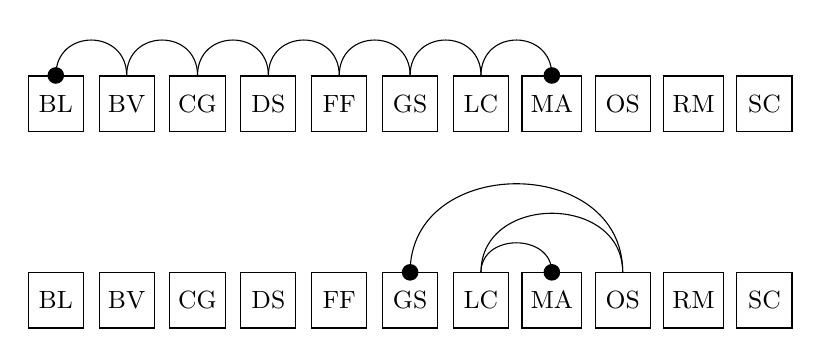
\begin{tikzpicture}[node distance=9mm, main node/.style={rectangle,draw,minimum size=7mm}]%
  \node at (0, 0) {};
  {\small
    \node[main node] (BL) {BL};
    \node[main node] (BV) [right of=BL] {BV};
    \node[main node] (CG) [right of=BV] {CG};
    \node[main node] (DS) [right of=CG] {DS};
    \node[main node] (FF) [right of=DS] {FF};
    \node[main node] (GS) [right of=FF] {GS};
    \node[main node] (LC) [right of=GS] {LC};
    \node[main node] (MA) [right of=LC] {MA};
    \node[main node] (OS) [right of=MA] {OS};
    \node[main node] (RM) [right of=OS] {RM};
    \node[main node] (SC) [right of=RM] {SC};
  }
  \draw [out=90,in=90,distance=0.6cm] (BL.north) to (BV.north);
  \draw [out=90,in=90,distance=0.6cm] (BV.north) to (CG.north);
  \draw [out=90,in=90,distance=0.6cm] (CG.north) to (DS.north);
  \draw [out=90,in=90,distance=0.6cm] (DS.north) to (FF.north);
  \draw [out=90,in=90,distance=0.6cm] (FF.north) to (GS.north);
  \draw [out=90,in=90,distance=0.6cm] (GS.north) to (LC.north);
  \draw [out=90,in=90,distance=0.6cm] (LC.north) to (MA.north);

  \fill (BL.north) circle [radius=3pt];
  \fill (MA.north) circle [radius=3pt];
  
  {\small
    \node[main node] (BL) at (0, -2.5) {BL};
    \node[main node] (BV) [right of=BL] {BV};
    \node[main node] (CG) [right of=BV] {CG};
    \node[main node] (DS) [right of=CG] {DS};
    \node[main node] (FF) [right of=DS] {FF};
    \node[main node] (GS) [right of=FF] {GS};
    \node[main node] (LC) [right of=GS] {LC};
    \node[main node] (MA) [right of=LC] {MA};
    \node[main node] (OS) [right of=MA] {OS};
    \node[main node] (RM) [right of=OS] {RM};
    \node[main node] (SC) [right of=RM] {SC};
  }

  \draw [out=90,in=90,distance=1.5cm] (GS.north) to (OS.north);
  \draw [out=90,in=90,distance=1cm] (OS.north) to (LC.north);
  \draw [out=90,in=90,distance=0.5cm] (LC.north) to (MA.north);

  \fill (GS.north) circle [radius=3pt];
  \fill (MA.north) circle [radius=3pt];
\end{tikzpicture}

